\section{Experimental Results}
\label{sec:experiments}
We first examine the computational speed of our PConv and its effectiveness when combined with a PWConv. We then comprehensively evaluate the performance of our FasterNet for classification, detection, and segmentation tasks. Finally, we conduct a brief ablation study. 

To benchmark the latency and throughput, we choose the following three typical processors, which cover a wide range of computational capacity: GPU (2080Ti), CPU (Intel i9-9900X, using a single thread), and ARM (Cortex-A72, using a single thread). We report their latency for inputs with a batch size of 1 and throughput for inputs with a batch size of 32. During inference, the BN layers are merged to their adjacent layers wherever applicable.

\subsection{PConv is fast with high FLOPS}
% Please add the following required packages to your document preamble:
% \usepackage{multirow}
% \usepackage{graphicx}
\begin{table*}
\centering
\resizebox{.82\textwidth}{!}{%
\setlength{\tabcolsep}{2pt}
\begin{tabular}{c|cc|cc|cc|cc}
\toprule
\multirow{2}{*}{\begin{tabular}[c]{@{}c@{}}Operator\end{tabular}} & \multirow{2}{*}{\begin{tabular}[c]{@{}c@{}}Feature map\\ size\end{tabular}} & \multirow{2}{*}{\begin{tabular}[c]{@{}c@{}}FLOPs (M), \\ $\times$10 layers\end{tabular}} & \multicolumn{2}{c|}{GPU} & \multicolumn{2}{c|}{CPU} & \multicolumn{2}{c}{ARM} \\
 &  &  & \small Throughput (fps) & \small FLOPS (G/s) & \small Latency (ms) & \small FLOPS (G/s) & \small Latency (ms) & \small FLOPS (G/s) \\ \midrule
\multirow{5}{*}{Conv 3$\times$3} & 96$\times$56$\times$56 & 2601 & 3010 & 7824 & 35.67 & 72.90 & 779.57 & 3.33 \\
 & 192$\times$28$\times$28 & 2601 & 4893 & 12717 & 28.41 & 91.53 & 619.64 & 4.19 \\
 & 384$\times$14$\times$14 & 2601 & 4558 & 11854 & 31.85 & 81.66 & 595.09 & 4.37 \\
 & 768$\times$7$\times$7 & 2601 & 3159 & 8212 & 62.71 & 41.47 & 662.17 & 3.92 \\ \cline{2-9} 
 &\multicolumn{2}{c|}{\cc Average} &\cc - & \cc{10151} &\cc - & \cc{71.89} &\cc - & \cc{3.95} \\ \midrule 
\multirow{5}{*}{\begin{tabular}[c]{@{}c@{}}GConv 3$\times$3 \\ (16 groups)\end{tabular}} & 96$\times$56$\times$56 & 162 & 2888 & 469 & 21.90 & 7.42 & 166.30 & 0.97 \\
 & 192$\times$28$\times$28 & 162 & 10811 & 1754 & 7.58 & 21.44 & 96.22 & 1.68 \\
 & 384$\times$14$\times$14 & 162 & 15534 & 2514 & 4.40 & 36.88 & 63.57 & 2.55 \\
 & 768$\times$7$\times$7 & 162 & 16000 & 2598 & 4.28 & 37.97 & 65.20 & 2.49 \\ \cline{2-9} 
 &\multicolumn{2}{c|}{\cc Average} &\cc - & \cc{1833} &\cc - & \cc{25.93} &\cc - & \cc{1.92} \\ \midrule 
\multirow{5}{*}{\begin{tabular}[c]{@{}c@{}}DWConv 3$\times$3\end{tabular}} & 96$\times$56$\times$56 & 27.09 & 11940 & 323 & 3.59 & 7.52 & 108.70 & 0.24 \\
 & 192$\times$28$\times$28 & 13.54 & 23358 & 315 & 1.97 & 6.86 & 82.01 & 0.16 \\
 & 384$\times$14$\times$14 & 6.77 & 46377 & 313 & 1.06 & 6.35 & 94.89 & 0.07 \\
 & 768$\times$7$\times$7 & 3.38 & 88889 & 302 & 0.68 & 4.93 & 150.89 & 0.02 \\ \cline{2-9} 
 &\multicolumn{2}{c|}{\cc Average} &\cc - & \cc{313} &\cc - & \cc{6.42} &\cc - & \cc{0.12} \\ \midrule 
\multirow{5}{*}{\begin{tabular}[c]{@{}c@{}}PConv 3$\times$3\\ (ours, with $r=\frac{1}{4}$)
\end{tabular}} & 96$\times$56$\times$56 & 162 & 9215 & 1493 & 5.46 & 29.67 & 85.30 & 1.90 \\
 & 192$\times$28$\times$28 & 162 & 14360 & 2326 & 3.09 & 52.43 & 66.46 & 2.44 \\
 & 384$\times$14$\times$14 & 162 & 24408 & 3954 & 3.58 & 45.25 & 49.98 & 3.24 \\
 & 768$\times$7$\times$7 & 162 & 32866 & 5324 & 5.02 & 32.27 & 48.30 & 3.35 \\ \cline{2-9} 
 &\multicolumn{2}{c|}{\cc Average} &\cc - &\cc{3274} &\cc - &\cc {39.91} &\cc - &\cc {2.73} \\ \bottomrule
\end{tabular}%
}
\vspace{-0.08in}
\caption{On-device FLOPS for different operations. PConv appears as an appealing choice for high FLOPS with reduced FLOPs.}
\label{FLOPS_compare}
\vspace{-0.15in}
\end{table*}

We below show that our PConv is fast and better exploits the on-device computational capacity. Specifically, we stack 10 layers of pure PConv and take feature maps of typical dimensions as inputs. We then measure FLOPs and latency/throughput on GPU, CPU, and ARM processors, which also allow us to further compute FLOPS. We repeat the same procedure for other convolutional variants and make comparisons. 

Results in~\cref{FLOPS_compare} show that PConv is overall an appealing choice for high FLOPS with reduced FLOPs. It has only $\frac{1}{16}$ FLOPs of a regular Conv and achieves $10.5\times$, $6.2\times$, and $22.8\times$ higher FLOPS than the DWConv on GPU, CPU, and ARM, respectively. We are unsurprised to see that the regular Conv has the highest FLOPS as it has been constantly optimized for years. However, its total FLOPs and latency/throughput are unaffordable. GConv and DWConv, despite their significant reduction in FLOPs, suffer from a drastic decrease in FLOPS. In addition, they tend to increase the number of channels to compensate for the performance drop, which, however, increase their latency.

\subsection{PConv is effective together with PWConv}
We next show that a PConv followed by a PWConv is effective in approximating a regular Conv to transform the feature maps. To this end, we first build four datasets by feeding the ImageNet-1k val split images into a pre-trained ResNet50, and extract the feature maps before and after the first Conv $3\times3$ in each of the four stages. Each feature map dataset is further spilt into the train (70\%), val (10\%), and test (20\%) subsets. We then build a simple network consisting of a PConv followed by a PWConv and train it on the feature map datasets with a mean squared error loss. For comparison, we also build and train networks for DWConv + PWConv and GConv + PWConv under the same setting.


\cref{tab:PConvPWConv} shows that PConv + PWConv achieve the lowest test loss, meaning that they better approximate a regular Conv in feature transformation. The results also suggest that it is sufficient and efficient to capture spatial features from only a part of the feature maps. PConv shows a great potential to be the new go-to choice in designing fast and effective neural networks.

% Please add the following required packages to your document preamble:
% \usepackage{booktabs}
% \usepackage{graphicx}
\begin{table}
\vspace{0.05in}
\centering
\resizebox{.9\linewidth}{!}{%
\setlength{\tabcolsep}{3pt}
\begin{tabular}{cccc}
\toprule
Stage & \small{DWConv+PWConv} & \begin{tabular}[c]{@{}c@{}}\small{GConv+PWConv} \\ (16 groups)\end{tabular} & \begin{tabular}[c]{@{}c@{}}\cc \small{PConv+PWConv}\\ \cc $r=\frac{1}{4}$\end{tabular} \\ \midrule
1       & 0.0089 & 0.0065 & \cc 0.0069          \\
2       & 0.0158 & 0.0137          & \cc{0.0136} \\
3       & 0.0214 & 0.0202          & \cc{0.0172} \\
4       & 0.0130 & 0.0128          & \cc{0.0115} \\ \midrule
Average & 0.0148 & 0.0133          & \cc{0.0123} \\ \bottomrule
\end{tabular}%
}
\vspace{-0.05in}
\caption{A PConv followed by a PWConv well approximates the regular Conv $3 \times 3$ at different stages of a pre-trained ResNet50. PConv + PWConv together have the lowest test loss on average.}
\label{tab:PConvPWConv}
\vspace{-0.15in}
\end{table}


\subsection{FasterNet on ImageNet-1k classification}

\begin{figure}
    \centering
    \vspace{-0.05in}
    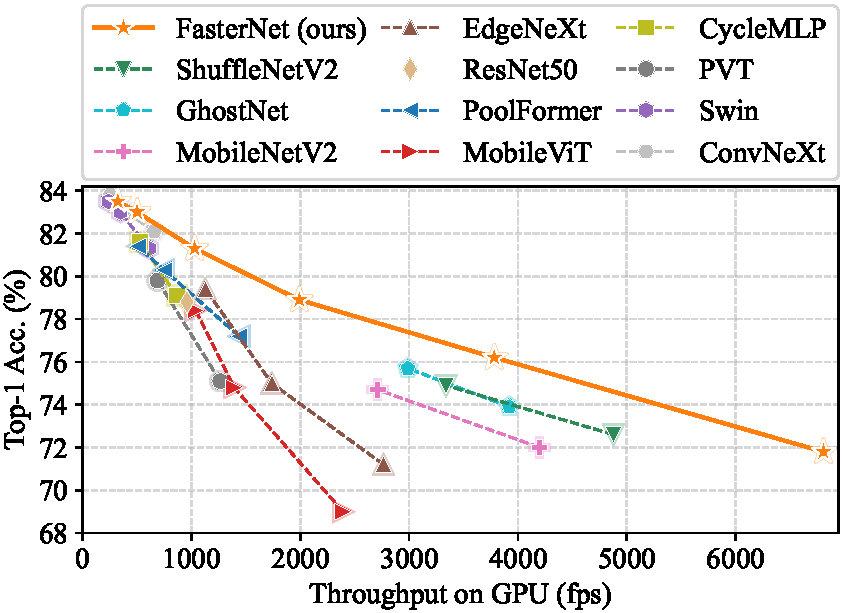
\includegraphics[width=1\linewidth]{figures/fps_latency_gpu_st-cropped.pdf}
    
    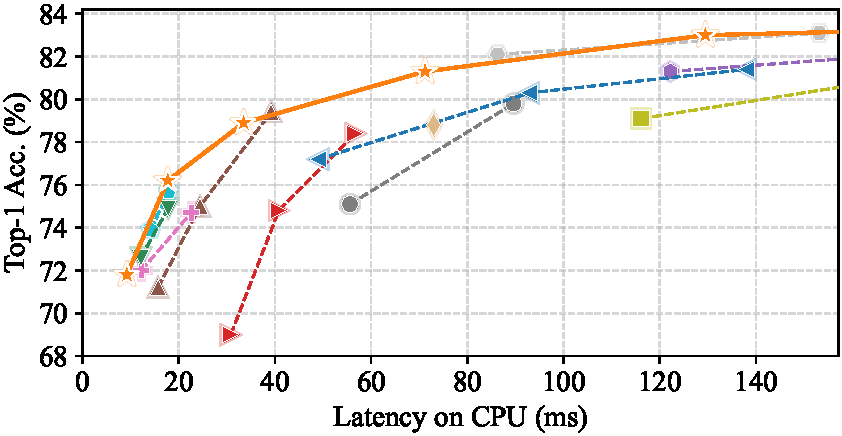
\includegraphics[width=1\linewidth]{figures/acc_latency_cpu_st-cropped.pdf}
    
    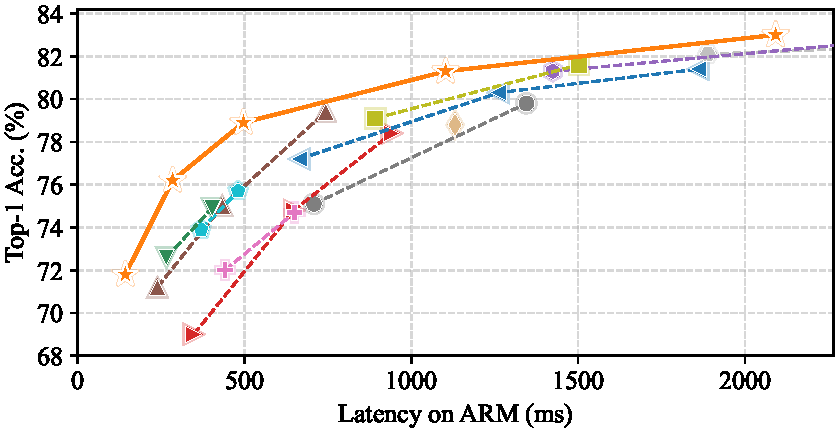
\includegraphics[width=1\linewidth]{figures/acc_latency_arm_st-cropped.pdf}
    
    \vspace{-0.15in}
    \caption{FasterNet has the highest efficiency in balancing accuracy-throughput and accuracy-latency trade-offs for different devices. To save space and make the plots more proportionate, we showcase network variants within a certain range of latency. Full plots can be found in the appendix, which show consistent results.}
    \label{fig:imageent}
    \vspace{-0.15in}
\end{figure}


    \begin{tabular}{c|clccccccc}
        \toprule
      General Arch.  &  Token Mixer    & Outcome Model    & Image Size & Params (M)  & MACs (G) & Top-1 (\%) \\
        \whline
    {\multirow{5}{*}{\makecell[c]{Convolutional \\ Neural Netowrks}}}  & \multirow{5}{*}{---}   & \resnetdot{} RSB-ResNet-18 \cite{resnet, resnet_improved} & 224 & 12 & 1.8 & 70.6 \\
         &   & \resnetdot{} RSB-ResNet-34 \cite{resnet, resnet_improved} & 224 & 22 & 3.7 & 75.5 \\
         &   & \resnetdot{} RSB-ResNet-50 \cite{resnet, resnet_improved} & 224 & 26 & 4.1 & 79.8 \\
         &   & \resnetdot{} RSB-ResNet-101 \cite{resnet, resnet_improved} & 224 &  45 & 7.9 & 81.3 \\
         &   & \resnetdot{} RSB-ResNet-152 \cite{resnet, resnet_improved} & 224 & 60 & 11.6 & 81.8 \\
        \hline
         
   \multirow{22}{*}{MetaFormer}  & \multirow{8}{*}{Attention} & \vitdot{} ViT-B/16$^*$ \cite{vit} & 224 &  86 & 17.6 & 79.7 \\
             &          & \vitdot{} ViT-L/16$^*$ \cite{vit} & 224 & 307 & 63.6 & 76.1 \\
             &          & \deitdot{} DeiT-S \cite{deit} & 224 & 22 & 4.6 & 79.8 \\
             &          & \deitdot{} DeiT-B \cite{deit} & 224 &  86 & 17.5 & 81.8 \\
             &          & \pvtdot{} PVT-Tiny \cite{pvt} & 224 & 13 & 1.9 & 75.1 \\
             &          & \pvtdot{} PVT-Small \cite{pvt} & 224 & 25 & 3.8 & 79.8 \\
             &          & \pvtdot{} PVT-Medium \cite{pvt} & 224 & 44 &  6.7 & 81.2 \\
             &          & \pvtdot{} PVT-Large \cite{pvt} & 224 & 61 &  9.8 & 81.7 \\
    \cline{2-7}
             & \multirow{9}{*}{Spatial MLP} & \mlpmixerdot{} MLP-Mixer-B/16 \cite{mlp-mixer} & 224 & 59 & 12.7 & 76.4 \\
             &             & \resmlp{} ResMLP-S12 \cite{resmlp} & 224 & 15 & 3.0 & 76.6 \\
             &             & \resmlp{} ResMLP-S24 \cite{resmlp} & 224 & 30 & 6.0 & 79.4 \\
             &             & \resmlp{} ResMLP-B24 \cite{resmlp} & 224 & 116 & 23.0 & 81.0 \\
             &             & \swinmixer{} Swin-Mixer-T/D24 \cite{swin} & 256 & 20 & 4.0 & 79.4 \\
             &             & \swinmixer{} Swin-Mixer-T/D6 \cite{swin} & 256 & 23 & 4.0 & 79.7 \\
             &             & \swinmixer{} Swin-Mixer-B/D24 \cite{swin} & 224 & 61 & 10.4 & 81.3 \\
             &             & \gmlp{} gMLP-S \cite{gmlp} & 224 & 20 & 4.5 & 79.6 \\
             &             & \gmlp{} gMLP-B \cite{gmlp} & 224 & 73 & 15.8 & 81.6 \\
    \cline{2-7}
             & \multirow{5}{*}{Pooling}  & \poolformer{} PoolFormer-S12 & 224 & 12 & 1.8 & 77.2 \\ % 77.3
             &         & \poolformer{} PoolFormer-S24 & 224 & 21 & 3.4 & 80.3 \\
             &         & \poolformer{} PoolFormer-S36 & 224 & 31 & 5.0 & 81.4 \\ % 81.5
             &         & \poolformer{} PoolFormer-M36 & 224 & 56 & 8.8 & 82.1 \\
             &         & \poolformer{} PoolFormer-M48 & 224 & 73 & 11.6 & 82.5 \\
    \bottomrule
             
    \end{tabular}
% Please add the following required packages to your document preamble:
% \usepackage{booktabs}
% \usepackage{graphicx}
% \usepackage[table,xcdraw]{xcolor}
% If you use beamer only pass "xcolor=table" option, i.e. \documentclass[xcolor=table]{beamer}
\begin{table*}
% \vspace{-0.05in}
\centering
\resizebox{.9\linewidth}{!}{%
\setlength{\tabcolsep}{5pt}
\begin{tabular}{lccccccccc}
\toprule
Backbone &
\begin{tabular}[c]{c}Params \\ (M)\end{tabular} &
\begin{tabular}[c]{c}FLOPs \\ (G)\end{tabular} &
\begin{tabular}[c]{c}Latency on\\GPU (ms)\end{tabular} &
\hspace{0.1cm} $AP^b$ \hspace{0.1cm}&
\hspace{0.1cm} $AP^b_{50}$ \hspace{0.1cm}&
\hspace{0.1cm} $AP^b_{75}$ \hspace{0.1cm}&
\hspace{0.1cm} $AP^m$ \hspace{0.1cm}&
\hspace{0.1cm} $AP^m_{50}$ \hspace{0.1cm}&
\hspace{0.1cm} $AP^m_{75}$ \hspace{0.1cm} \\ \midrule
ResNet50~\cite{he2016deep}        & 44.2  & 253   & 54.9  & 38.0 & 58.6 & 41.4 & 34.4 & 55.1 & 36.7 \\
PoolFormer-S24~\cite{yu2022metaformer}    & 41.0  & 233   & 111.0 & 40.1 & 62.2 & 43.4 & 37.0 & 59.1 & 39.6 \\
PVT-Small~\cite{wang2021pyramid}        & 44.1  & 238   & 89.5  & 40.4 & 62.9 & 43.8 & 37.8 & 60.1 & 40.3 \\
\cc FasterNet-S      &\cc 49.0  &\cc 258   &\cc 54.3  &\cc 39.9 &\cc 61.2 &\cc 43.6 &\cc 36.9 &\cc 58.1 &\cc 39.7 \\ \midrule
ResNet101~\cite{he2016deep}       & 63.2  & 329   & 68.9  & 40.4 & 61.1 & 44.2 & 36.4 & 57.7 & 38.8 \\
ResNeXt101-32$\times$4d~\cite{xie2017aggregated} & 62.8  & 333   & 80.5  & 41.9 & 62.5 & 45.9 & 37.5 & 59.4 & 40.2 \\
PoolFormer-S36~\cite{yu2022metaformer}    & 50.5  & 266   & 146.9 & 41.0 & 63.1 & 44.8 & 37.7 & 60.1 & 40.0 \\
PVT-Medium~\cite{wang2021pyramid}       & 63.9  & 295   & 117.3 & 42.0 & 64.4 & 45.6 & 39.0 & 61.6 & 42.1 \\
\cc FasterNet-M      &\cc 71.2  &\cc 344   &\cc 71.4  &\cc 43.0 &\cc 64.4 &\cc 47.4 &\cc 39.1 &\cc 61.5 &\cc 42.3 \\ \midrule
ResNeXt101-64$\times$4d~\cite{xie2017aggregated} & 101.9 & 487   & 112.9 & 42.8 & 63.8 & 47.3 & 38.4 & 60.6 & 41.3 \\
PVT-Large~\cite{wang2021pyramid}        & 81.0  & 358   & 152.2 & 42.9 & 65.0 & 46.6 & 39.5 & 61.9 & 42.5 \\
\cc FasterNet-L      &\cc 110.9 &\cc 484 &\cc 93.8  &\cc 44.0 &\cc 65.6 &\cc 48.2 &\cc 39.9 &\cc 62.3 &\cc 43.0 \\ \bottomrule
\end{tabular}%
}
\vspace{-0.08in}
\caption{Results on COCO object detection and instance segmentation benchmarks. FLOPs are calculated with image size (1280, 800).}
\label{tab:coco}
\vspace{-0.1in}
\end{table*}
% Please add the following required packages to your document preamble:
% \usepackage{booktabs}
% \usepackage{multirow}
\begin{table}
\centering
% \vspace{-0.05in}
\resizebox{1.\linewidth}{!}{%
\setlength{\tabcolsep}{1pt}
\begin{tabular}{llcccc}
\toprule
Ablation&
Variant &
\begin{tabular}[c]{@{}c@{}} {\small Throughput}  \\ on {\small GPU} \\ (fps)\end{tabular} &
\begin{tabular}[c]{@{}c@{}} {\small Latency} \\ on {\small CPU} \\ (ms)\end{tabular} &
\begin{tabular}[c]{@{}c@{}} {\small Latency} \\ on {\small ARM} \\ (ms)\end{tabular} &
\begin{tabular}[c]{@{}c@{}}Acc. \\ (\%)\end{tabular} \\ \midrule
\multirow{3}{*}{Partial ratio} & $\text{T0}^*$ w/  $r = 1/2$   &6626       & 9.6       & 145       & 71.7      \\
                               &\cc T0 w/ $r = 1/4$ &\cc 6807   &\cc 9.2    &\cc 143    &\cc 71.9   \\
                               & $\text{T0}^*$ w/ $r = 1/8$    &6204	     &8.9        &140        & 71.3    \\ \midrule
\multirow{2}{*}{Normalization} &\cc T0 w/ BN          &\cc 6807   &\cc 9.2    &\cc 143 &\cc 71.9                   \\
                               & T0 w/ LN          &5515	  &10.7 &159                         & 71.9                     \\ \midrule
\multirow{5}{*}{Activation}    & T0 w/ ReLU        &6929	  &8.2  &114                         & 71.3                     \\
                               &$\text{T0}^*$ w/ ReLU        & 5866                 & 9.3                  & 143 & 71.7 \\
                               &\cc T0 w/ GELU        &\cc 6807   &\cc 9.2    &\cc 143 &\cc 71.9                     \\
                               &\cc T2 w/ ReLU        &\cc 1991                 &\cc 33.5                 &\cc 497 &\cc 78.9                     \\
                               & T2 w/ GELU        &1985	  &35.4  &557                         & 78.7 \\ 
\bottomrule
\end{tabular}%
}
\vspace{-0.1in}
\caption{Ablation on the partial ratio, normalization, and activation of FasterNet. Rows highlighted in grey are the default settings. $\text{T0}^*$ denotes T0 variants with modified network width and depth.}
\label{tab:ablation}
\vspace{-0.1in}
\end{table}


To verify the effectiveness and efficiency of our FasterNet, we first conduct experiments on the large-scale ImageNet-1k classification dataset~\cite{russakovsky2015imagenet}. It covers 1k categories of common objects and contains about 1.3M labeled images for training and 50k labeled images for validation. We train our models for 300 epochs using AdamW optimizer~\cite{loshchilov2017decoupled}. We set the batch size to 2048 for the FasterNet-M/L and 4096 for other variants. We use cosine learning rate scheduler~\cite{loshchilov2016sgdr} with a peak value of $0.001\cdot\text{batch size}/1024$ and a 20-epoch linear warmup. We apply commonly-used regularization and augmentation techniques, including Weight Decay~\cite{krogh1991simple}, Stochastic Depth~\cite{huang2016deep}, Label Smoothing~\cite{szegedy2016rethinking}, Mixup~\cite{zhang2017mixup}, Cutmix~\cite{yun2019cutmix} and Rand Augment~\cite{cubuk2020randaugment}, with varying magnitudes for different FasterNet variants. To reduce the training time, we use $192 \times 192$ resolution for the first 280 training epochs and $224 \times 224$ for the remaining 20 epochs. For fair comparison, we do not use knowledge distillation~\cite{hinton2015distilling} and neural architecture search~\cite{zoph2016neural}. We report our top-1 accuracy on the validation set with a center crop at $224 \times 224$ resolution and a 0.9 crop ratio. Detailed training and validation settings are provided in the appendix.

\cref{fig:imageent} and \cref{tab:imagenet} demonstrate the superiority of our FasterNet over state-of-the-art classification models. The trade-off curves in~\cref{fig:imageent} clearly show that FasterNet sets the new state-of-the-art in balancing accuracy and latency/throughput among all the networks examined. From another perspective, FasterNet runs faster than various CNN, ViT and MLP models on a wide range of devices, when having similar top-1 accuracy. As quantitatively shown in~\cref{tab:imagenet}, FasterNet-T0 is $2.8\times$, $3.3\times$, and $2.4\times$
faster than MobileViT-XXS~\cite{mehta2021mobilevit} on GPU, CPU, and ARM processors, respectively, while being 2.9\% more accurate.
Our large FasterNet-L achieves 83.5\% top-1 accuracy, comparable to the emerging Swin-B~\cite{liu2021swin} and ConvNeXt-B~\cite{liu2022convnet} while having 36\% and 28\% higher inference throughput on GPU, as well as saving 37\% and 15\% compute time on CPU. Given such promising results, we highlight that our FasterNet is much simpler than many other models in terms of architectural design, which showcases the feasibility of designing simple yet powerful neural networks.


\subsection{FasterNet on downstream tasks}
To further evaluate the generalization ability of FasterNet, we conduct experiments on the challenging COCO dataset~\cite{lin2014microsoft} for object detection and instance segmentation. As a common practice, we employ the ImageNet pre-trained FasterNet as a backbone and equip it with the popular Mask R-CNN detector~\cite{he2017mask}. To highlight the effectiveness of the backbone itself, we simply follow PoolFormer~\cite{yu2022metaformer} and adopt an AdamW optimizer, a $1 \times$ training schedule (12 epochs), a batch size of 16, and other training settings without further hyper-parameter tuning.

\cref{tab:coco} shows the results for comparison between FasterNet and representative models. FasterNet consistently outperforms ResNet and ResNext by having higher average precision (AP) with similar latency. Specifically, FasterNet-S yields $+1.9$ higher box AP and $+2.4$ higher mask AP compared to the standard baseline ResNet50. FasterNet is also competitive against the ViT variants. Under similar FLOPs, FasterNet-L reduces PVT-Large's latency by 38\%, \ie, from 152.2 ms to 93.8 ms on GPU, and achieves $+1.1$ higher box AP and $+0.4$ higher mask AP.

\subsection{Ablation study}
We conduct a brief ablation study on the value of partial ratio $r$ and the choices of activation and normalization layers. We compare different variants in terms of ImageNet top-1 accuracy and on-device latency/throughput. Results are summarized in~\cref{tab:ablation}. For the partial ratio $r$, we set it to $\frac{1}{4}$ for all FasterNet variants by default, which achieves higher accuracy, higher throughput, and lower latency at similar complexity. A too large partial ratio $r$ would make PConv degrade to a regular Conv, while a too small value would render PConv less effective in capturing the spatial features. 
For the normalization layers, we choose BatchNorm over LayerNorm because BatchNorm can be merged into its adjacent convolutional layers for faster inference while it is as effective as LayerNorm in our experiment.
For the activation function, interestingly, we empirically found that GELU fits FasterNet-T0/T1 models more efficiently than ReLU. It, however, becomes opposite for FasterNet-T2/S/M/L. Here we only show two examples in~\cref{tab:ablation} due to space constraint. We conjecture that GELU strengthens FasterNet-T0/T1 by having higher non-linearity, while the benefit fades away for larger FasterNet variants.